\documentclass{article}
\usepackage{pgfplots}
\pgfplotsset{compat=1.18}

\begin{document}

\begin{figure}[h]
    \centering
    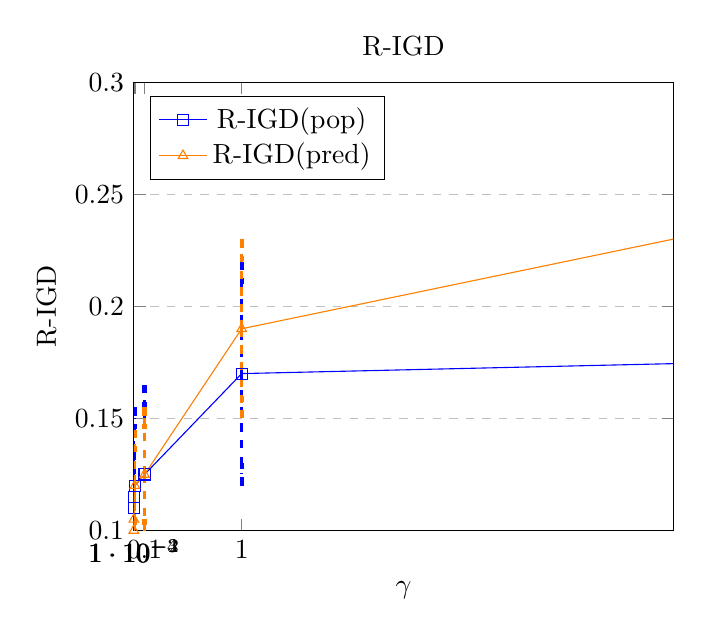
\begin{tikzpicture}
        \begin{axis}[
            title={R-IGD},
            xlabel={$\gamma$},
            ylabel={R-IGD},
            xmin=0.0001, xmax=5,
            ymin=0.1, ymax=0.3,
            xtick={0.0001, 0.001, 0.01, 0.1, 1, 10},
            ytick={0.1, 0.15, 0.2, 0.25, 0.3},
            legend pos=north west,
            ymajorgrids=true,
            grid style=dashed,
        ]
        
        % Line for R-IGD(pop)
        \addplot[
            color=blue,
            mark=square,
            error bars/.cd,
            y dir=both,
            y explicit,
            error bar style={line width=1pt, dashed, fill=blue!20},
            error mark options={line width=1.5pt, mark size=4pt},
        ]
        coordinates {
            (0.0001, 0.11) +-(0, 0.02)
            (0.001, 0.115) +-(0, 0.025)
            (0.01, 0.12) +-(0, 0.03)
            (0.1, 0.125) +-(0, 0.035)
            (1, 0.17) +-(0, 0.045)
            (10, 0.18) +-(0, 0.05)
        };
        \addlegendentry{R-IGD(pop)}
        
        % Line for R-IGD(pred)
        \addplot[
            color=orange,
            mark=triangle,
            error bars/.cd,
            y dir=both,
            y explicit,
            error bar style={line width=1pt, dashed, fill=orange!20},
            error mark options={line width=1.5pt, mark size=4pt},
        ]
        coordinates {
            (0.0001, 0.1) +-(0, 0.01)
            (0.001, 0.105) +-(0, 0.015)
            (0.01, 0.12) +-(0, 0.02)
            (0.1, 0.125) +-(0, 0.025)
            (1, 0.19) +-(0, 0.035)
            (10, 0.28) +-(0, 0.04)
        };
        \addlegendentry{R-IGD(pred)}
        
        \end{axis}
    \end{tikzpicture}
    \caption{(a) The value of R-IGD calculated on the population from the last iteration and the predictions given by the model. The area within one standard deviation is shaded.\newline
             (b) The variance of decision variables of the predictions. The model's predictions converge to a small area as $\gamma$ increases.}
    \label{fig:rigd_performance}
\end{figure}

\end{document}